\documentclass{standalone}
\usepackage{tikz}

\begin{document}

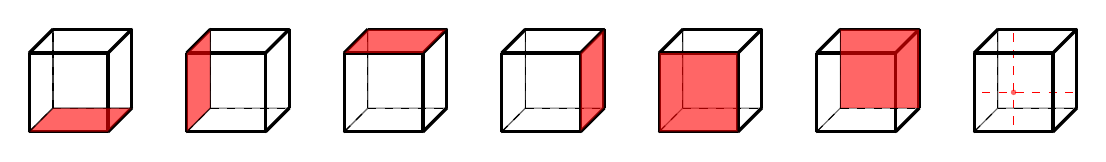
\begin{tikzpicture}
    \coordinate (A1) at (0, 0);
    \coordinate (A2) at (0, 1);
    \coordinate (A3) at (1, 1);
    \coordinate (A4) at (1, 0);
    \coordinate (B1) at (0.3, 0.3);
    \coordinate (B2) at (0.3, 1.3);
    \coordinate (B3) at (1.3, 1.3);
    \coordinate (B4) at (1.3, 0.3);

    \draw[very thick] (A1) -- (A2);
    \draw[very thick] (A2) -- (A3);
    \draw[very thick] (A3) -- (A4);
    \draw[very thick] (A4) -- (A1);

    \draw[dashed] (A1) -- (B1);
    \draw[dashed] (B1) -- (B2);
    \draw[very thick] (A2) -- (B2);
    \draw[very thick] (B2) -- (B3);
    \draw[very thick] (A3) -- (B3);
    \draw[very thick] (A4) -- (B4);
    \draw[very thick] (B4) -- (B3);
    \draw[dashed] (B1) -- (B4);

    \draw[opacity=0.6] (A1) -- (B1) -- (B4) -- (A4);
    \draw[opacity=0.5] (A1) -- (A2) -- (A3) -- (A4);
    \draw[opacity=0.6] (A1) -- (A2) -- (B2) -- (B1);
    \draw[opacity=0.6] (B1) -- (B2) -- (B3) -- (B4);
    \draw[opacity=0.6] (A3) -- (B3) -- (B4) -- (A4);
    \draw[opacity=0.6] (A2) -- (B2) -- (B3) -- (A3);

    \node[circle, fill, inner sep=0pt,minimum size=1pt] at (0, 0) {};
    \node[circle, fill, inner sep=0pt,minimum size=1pt] at (1, 0) {};
    \node[circle, fill, inner sep=0pt,minimum size=1pt] at (0, 1) {};
    \node[circle, fill, inner sep=0pt,minimum size=1pt] at (0.3, 1.3) {};
    \node[circle, fill, inner sep=0pt,minimum size=1pt] at (1.3, 1.3) {};
    \node[circle, fill, inner sep=0pt,minimum size=1pt] at (1.3, 0.3) {};

    \draw[fill=red, opacity=0.6] (A1) -- (B1) -- (B4) -- (A4);

    \coordinate (C1) at (2, 0);
    \coordinate (C2) at (2, 1);
    \coordinate (C3) at (3, 1);
    \coordinate (C4) at (3, 0);
    \coordinate (D1) at (2.3, 0.3);
    \coordinate (D2) at (2.3, 1.3);
    \coordinate (D3) at (3.3, 1.3);
    \coordinate (D4) at (3.3, 0.3);

    \draw[very thick] (C1) -- (C2);
    \draw[very thick] (C2) -- (C3);
    \draw[very thick] (C3) -- (C4);
    \draw[very thick] (C4) -- (C1);

    \draw[dashed] (C1) -- (D1);
    \draw[dashed] (D1) -- (D2);
    \draw[very thick] (C2) -- (D2);
    \draw[very thick] (D2) -- (D3);
    \draw[very thick] (C3) -- (D3);
    \draw[very thick] (C4) -- (D4);
    \draw[very thick] (D4) -- (D3);
    \draw[dashed] (D1) -- (D4);

    \draw[opacity=0.6] (C1) -- (D1) -- (D4) -- (C4);
    \draw[opacity=0.5] (C1) -- (C2) -- (C3) -- (C4);
    \draw[opacity=0.6] (C1) -- (C2) -- (D2) -- (D1);
    \draw[opacity=0.6] (D1) -- (D2) -- (D3) -- (D4);
    \draw[opacity=0.6] (C3) -- (D3) -- (D4) -- (C4);
    \draw[opacity=0.6] (C2) -- (D2) -- (D3) -- (C3);

    \node[circle, fill, inner sep=0pt,minimum size=1pt] at (2, 0) {};
    \node[circle, fill, inner sep=0pt,minimum size=1pt] at (3, 0) {};
    \node[circle, fill, inner sep=0pt,minimum size=1pt] at (2, 1) {};
    \node[circle, fill, inner sep=0pt,minimum size=1pt] at (2.3, 1.3) {};
    \node[circle, fill, inner sep=0pt,minimum size=1pt] at (3.3, 1.3) {};
    \node[circle, fill, inner sep=0pt,minimum size=1pt] at (3.3, 0.3) {};

    \draw[fill=red, opacity=0.6] (C1) -- (D1) -- (D2) -- (C2);


    \coordinate (E1) at (4, 0);
    \coordinate (E2) at (4, 1);
    \coordinate (E3) at (5, 1);
    \coordinate (E4) at (5, 0);
    \coordinate (F1) at (4.3, 0.3);
    \coordinate (F2) at (4.3, 1.3);
    \coordinate (F3) at (5.3, 1.3);
    \coordinate (F4) at (5.3, 0.3);

    \draw[very thick] (E1) -- (E2);
    \draw[very thick] (E2) -- (E3);
    \draw[very thick] (E3) -- (E4);
    \draw[very thick] (E4) -- (E1);

    \draw[dashed] (E1) -- (F1);
    \draw[dashed] (F1) -- (F2);
    \draw[very thick] (E2) -- (F2);
    \draw[very thick] (F2) -- (F3);
    \draw[very thick] (E3) -- (F3);
    \draw[very thick] (E4) -- (F4);
    \draw[very thick] (F4) -- (F3);
    \draw[dashed] (F1) -- (F4);

    \draw[opacity=0.6] (E1) -- (F1) -- (F4) -- (E4);
    \draw[opacity=0.5] (E1) -- (E2) -- (E3) -- (E4);
    \draw[opacity=0.6] (E1) -- (E2) -- (F2) -- (F1);
    \draw[opacity=0.6] (F1) -- (F2) -- (F3) -- (F4);
    \draw[opacity=0.6] (E3) -- (F3) -- (F4) -- (E4);
    \draw[opacity=0.6] (E2) -- (F2) -- (F3) -- (E3);


    \node[circle, fill, inner sep=0pt,minimum size=1pt] at (4, 0) {};
    \node[circle, fill, inner sep=0pt,minimum size=1pt] at (5, 0) {};
    \node[circle, fill, inner sep=0pt,minimum size=1pt] at (4, 1) {};
    \node[circle, fill, inner sep=0pt,minimum size=1pt] at (5.3, 1.3) {};
    \node[circle, fill, inner sep=0pt,minimum size=1pt] at (5.3, 1.3) {};
    \node[circle, fill, inner sep=0pt,minimum size=1pt] at (5.3, 0.3) {};

    \draw[fill=red, opacity=0.6] (E2) -- (F2) -- (F3) -- (E3);

    \coordinate (G1) at (6, 0);
    \coordinate (G2) at (6, 1);
    \coordinate (G3) at (7, 1);
    \coordinate (G4) at (7, 0);
    \coordinate (H1) at (6.3, 0.3);
    \coordinate (H2) at (6.3, 1.3);
    \coordinate (H3) at (7.3, 1.3);
    \coordinate (H4) at (7.3, 0.3);

    \draw[very thick] (G1) -- (G2);
    \draw[very thick] (G2) -- (G3);
    \draw[very thick] (G3) -- (G4);
    \draw[very thick] (G4) -- (G1);

    \draw[dashed] (G1) -- (H1);
    \draw[dashed] (H1) -- (H2);
    \draw[very thick] (G2) -- (H2);
    \draw[very thick] (H2) -- (H3);
    \draw[very thick] (G3) -- (H3);
    \draw[very thick] (G4) -- (H4);
    \draw[very thick] (H4) -- (H3);
    \draw[dashed] (H1) -- (H4);

    \draw[opacity=0.6] (G1) -- (H1) -- (H4) -- (G4);
    \draw[opacity=0.5] (G1) -- (G2) -- (G3) -- (G4);
    \draw[opacity=0.6] (G1) -- (G2) -- (H2) -- (H1);
    \draw[opacity=0.6] (H1) -- (H2) -- (H3) -- (H4);
    \draw[opacity=0.6] (G3) -- (H3) -- (H4) -- (G4);
    \draw[opacity=0.6] (G2) -- (H2) -- (H3) -- (G3);

    
\node[circle, fill, inner sep=0pt,minimum size=1pt] at (6, 0) {};
    
\node[circle, fill, inner sep=0pt,minimum size=1pt] at (7, 0) {};
    
\node[circle, fill, inner sep=0pt,minimum size=1pt] at (6, 1) {};
    
\node[circle, fill, inner sep=0pt,minimum size=1pt] at (6.3, 1.3) {};
    
\node[circle, fill, inner sep=0pt,minimum size=1pt] at (7.3, 1.3) {};
    
\node[circle, fill, inner sep=0pt,minimum size=1pt] at (7.3, 0.3) {};

    \draw[fill=red, opacity=0.6] (G3) -- (H3) -- (H4) -- (G4);

    \coordinate (I1) at (8, 0);
    \coordinate (I2) at (8, 1);
    \coordinate (I3) at (9, 1);
    \coordinate (I4) at (9, 0);
    \coordinate (J1) at (8.3, 0.3);
    \coordinate (J2) at (8.3, 1.3);
    \coordinate (J3) at (9.3, 1.3);
    \coordinate (J4) at (9.3, 0.3);

    \draw[very thick] (I1) -- (I2);
    \draw[very thick] (I2) -- (I3);
    \draw[very thick] (I3) -- (I4);
    \draw[very thick] (I4) -- (I1);

    \draw[dashed] (I1) -- (J1);
    \draw[dashed] (J1) -- (J2);
    \draw[very thick] (I2) -- (J2);
    \draw[very thick] (J2) -- (J3);
    \draw[very thick] (I3) -- (J3);
    \draw[very thick] (I4) -- (J4);
    \draw[very thick] (J4) -- (J3);
    \draw[dashed] (J1) -- (J4);

    \draw[opacity=0.6] (I1) -- (J1) -- (J4) -- (I4);
    \draw[opacity=0.5] (I1) -- (I2) -- (I3) -- (I4);
    \draw[opacity=0.6] (I1) -- (I2) -- (J2) -- (J1);
    \draw[opacity=0.6] (J1) -- (J2) -- (J3) -- (J4);
    \draw[opacity=0.6] (I3) -- (J3) -- (J4) -- (I4);
    \draw[opacity=0.6] (I2) -- (J2) -- (J3) -- (I3);

    \node[circle, fill, inner sep=0pt,minimum size=1pt] at (8, 0) {};
    \node[circle, fill, inner sep=0pt,minimum size=1pt] at (9, 0) {};
    \node[circle, fill, inner sep=0pt,minimum size=1pt] at (8, 1) {};
    \node[circle, fill, inner sep=0pt,minimum size=1pt] at (8.3, 1.3) {};
    \node[circle, fill, inner sep=0pt,minimum size=1pt] at (9.3, 1.3) {};
    \node[circle, fill, inner sep=0pt,minimum size=1pt] at (9.3, 0.3) {};

    \draw[fill=red, opacity=0.6] (I3) -- (I4) -- (I1) -- (I2);

    \coordinate (K1) at (10, 0);
    \coordinate (K2) at (10, 1);
    \coordinate (K3) at (11, 1);
    \coordinate (K4) at (11, 0);
    \coordinate (L1) at (10.3, 0.3);
    \coordinate (L2) at (10.3, 1.3);
    \coordinate (L3) at (11.3, 1.3);
    \coordinate (L4) at (11.3, 0.3);

    \draw[very thick] (K1) -- (K2);
    \draw[very thick] (K2) -- (K3);
    \draw[very thick] (K3) -- (K4);
    \draw[very thick] (K4) -- (K1);

    \draw[dashed] (K1) -- (L1);
    \draw[dashed] (L1) -- (L2);
    \draw[very thick] (K2) -- (L2);
    \draw[very thick] (L2) -- (L3);
    \draw[very thick] (K3) -- (L3);
    \draw[very thick] (K4) -- (L4);
    \draw[very thick] (L4) -- (L3);
    \draw[dashed] (L1) -- (L4);

    \draw[opacity=0.6] (K1) -- (L1) -- (L4) -- (K4);
    \draw[opacity=0.5] (K1) -- (K2) -- (K3) -- (K4);
    \draw[opacity=0.6] (K1) -- (K2) -- (L2) -- (L1);
    \draw[opacity=0.6] (L1) -- (L2) -- (L3) -- (L4);
    \draw[opacity=0.6] (K3) -- (L3) -- (L4) -- (K4);
    \draw[opacity=0.6] (K2) -- (L2) -- (L3) -- (K3);

    \node[circle, fill, inner sep=0pt,minimum size=1pt] at (10, 0) {};
    \node[circle, fill, inner sep=0pt,minimum size=1pt] at (11, 0) {};
    \node[circle, fill, inner sep=0pt,minimum size=1pt] at (10, 1) {};
    \node[circle, fill, inner sep=0pt,minimum size=1pt] at (10.3, 1.3) {};
    \node[circle, fill, inner sep=0pt,minimum size=1pt] at (11.3, 1.3) {};
    \node[circle, fill, inner sep=0pt,minimum size=1pt] at (11.3, 0.3) {};

    \draw[fill=red, opacity=0.6] (L1) -- (L2) -- (L3) -- (L4);

    \coordinate (M1) at (12, 0);
    \coordinate (M2) at (12, 1);
    \coordinate (M3) at (13, 1);
    \coordinate (M4) at (13, 0);
    \coordinate (N1) at (12.3, 0.3);
    \coordinate (N2) at (12.3, 1.3);
    \coordinate (N3) at (13.3, 1.3);
    \coordinate (N4) at (13.3, 0.3);

    \draw[dashed, red] (12.5, 1.25) -- (12.5, 0);
    \draw[dashed, red] (12.1, 0.5) -- (13.25, 0.5);
    \draw[very thick] (M1) -- (M2);
    \draw[very thick] (M2) -- (M3);
    \draw[very thick] (M3) -- (M4);
    \draw[very thick] (M4) -- (M1);

    \draw[dashed] (M1) -- (N1);
    \draw[dashed] (N1) -- (N2);
    \draw[very thick] (M2) -- (N2);
    \draw[very thick] (N2) -- (N3);
    \draw[very thick] (M3) -- (N3);
    \draw[very thick] (M4) -- (N4);
    \draw[very thick] (N4) -- (N3);
    \draw[dashed] (N1) -- (N4);

    \draw[opacity=0.6] (M1) -- (N1) -- (N4) -- (M4);
    \draw[opacity=0.5] (M1) -- (M2) -- (M3) -- (M4);
    \draw[opacity=0.6] (M1) -- (M2) -- (N2) -- (N1);
    \draw[opacity=0.6] (N1) -- (N2) -- (N3) -- (N4);
    \draw[opacity=0.6] (M3) -- (N3) -- (N4) -- (M4);
    \draw[opacity=0.6] (M2) -- (N2) -- (N3) -- (M3);

    \node[circle, fill, inner sep=0pt,minimum size=1pt] at (12, 0) {};
    \node[circle, fill, inner sep=0pt,minimum size=1pt] at (13, 0) {};
    \node[circle, fill, inner sep=0pt,minimum size=1pt] at (12, 1) {};
    \node[circle, fill, inner sep=0pt,minimum size=1pt] at (12.3, 1.3) {};
    \node[circle, fill, inner sep=0pt,minimum size=1pt] at (13.3, 1.3) {};
    \node[circle, fill, inner sep=0pt,minimum size=1pt] at (13.3, 0.3) {};

    \node[circle, fill=red, inner sep=0pt,minimum size=2pt, opacity=0.6] at (12.5, 0.5) {};

\end{tikzpicture}

\end{document}